% Class def
\documentclass[xcolor=table,serif]{beamer} 
% %Language and accents
\usepackage[spanish]{babel}
\usepackage[utf8]{inputenc}
% For text justification
\usepackage{ragged2e}
% ams math packages
\usepackage{amsmath}
\usepackage{amsfonts}
\usepackage{amssymb}
% % Images 
 \usepackage{graphicx}
 \usepackage{subfigure}
 \usepackage[labelformat=empty]{caption}
 \setbeamerfont{caption}{size=\scriptsize}
% theme 
\usetheme[]{Madrid}
%\usepackage{colortbl}
%\usepackage[table]{xcolor} 
\usepackage{multimedia}
\usepackage{subfigure}
%\usetheme{Boadilla} 
%\usecolortheme{dolphin} 
\graphicspath{{img/}}
% Links and hyperlinks
 \usepackage{url}
% \usepackage{hyperref}
 \hypersetup{colorlinks, linkcolor = blue, urlcolor = blue}
% Default fixed font does not support bold face
\DeclareFixedFont{\ttb}{T1}{txtt}{bx}{n}{8} % for bold
\DeclareFixedFont{\ttm}{T1}{txtt}{m}{n}{8}  % for normal
% For text boxes
\usepackage{fancybox}
% Custom colors
\usepackage{color}
\definecolor{deepblue}{rgb}{0,0,0.5}
\definecolor{deepred}{rgb}{0.6,0,0}
\definecolor{deepgreen}{rgb}{0,0.5,0}

\usepackage{listings}

% Python style for highlighting
\newcommand\pythonstyle{\lstset{
language=Python,
basicstyle=\ttm,
otherkeywords={self},             % Add keywords here
keywordstyle=\ttb\color{deepblue},
emph={MyClass,__init__},          % Custom highlighting
emphstyle=\ttb\color{deepred},    % Custom highlighting style
stringstyle=\color{deepgreen},
frame=tb,                         % Any extra options here
showstringspaces=false            % 
}}
% Python environment
\lstnewenvironment{python}[1][]
{
\pythonstyle
\lstset{#1}
}
{}

\date{\today} 
\logo{Ingeniería Física\includegraphics[width=1cm]{eafit_escudo}} 
\author[]{Santiago Echeverri Chac\'on\\ Asesor: \\ Nicol\'as Guar\'in Zapata}
\title[Trabajo de grado]{Una plataforma para la simulación de propagación de luz en estructuras fotónicas cristalinas con defectos.}
\subtitle{Trabajo de grado}
\institute{Universidad EAFIT}

\begin{document}

\begin{frame}
\titlepage
\end{frame}
\AtBeginSection[]
		{
			 \begin{frame}
			  \frametitle{Contenido}
			  \small
		  	\tableofcontents[currentsection]%,hideothersubsections]
			  \normalsize
 			\end{frame}
		}
\section{Introducción}
		
	\subsection{Planteamiento del Problema}
	\begin{frame}
	\frametitle{Planteamiento del problema}
	\justifying
	En el trabajo que se presenta aquí se propuso construir un paquete de herramientas de software que permitiera el análisis de propagación de campos electromagnéticos en el contexto de cristales fotónicos (PCs), con la capacidad de modelar defectos.  \\
	\pause
	Esta presentación se propone responder las siguientes preguntas:
	\vskip20pt
	\begin{columns}[t]
		\column{0.2 \textwidth}
				\shadowbox{¿Por qué?}
		\column{0.2 \textwidth}
				\shadowbox{¿Para qué?}
		\column{0.2 \textwidth}
				\shadowbox{¿Cómo?}
	\end{columns}

	\end{frame}
	\begin{frame}
	\frametitle{Objetivos planteados en el anteproyecto}
		\begin{block}{Objetivo General}
		\begin{itemize}
			\pause
			\item Construir una plataforma de software capaz de simular propagación de campos electromagnéticos en PCs con defectos tales como cavidades e inclusiones.
			\pause
			\item La arquitectura de la plataforma debe ser diseñada de tal forma que se faciliten: 
			\begin{itemize}
				\pause
				\item las futuras actualizaciones,
				\pause
				\item soporte de esquemas de optimización,
				\pause
				\item e integración con otros tipos de simulaciones como aquellas de confinamiento de electrones en pozos de potencial y cristales. 	
			\end{itemize}
		\end{itemize}
		\end{block}
		\end{frame}
		\begin{frame}
		\begin{block}{Objetivos Espec\'ificos}
	    \pause
	    \begin{enumerate}
			\item  Adquirir la teoría detrás de los campos electromagnéticos y sus aplicaciones en el contexto de cristales fotónicos. Particularmente: 
			\pause
			\begin{enumerate}
				\item Detalles sobre la modelación de cristales fotónicos y las herramientas matemáticas con las que se define la periodicidad, así como \pause
	 			\item  una visión global de los métodos computacionales en electromagnetismo y un entendimiento más profundo de los métodos que mejor se ajustan a la definición del problema.
	 		\end{enumerate}
			\pause
			\item Definir un conjunto de requerimientos de implementación. 
			\pause
			\item Programar los algoritmos que solucionen los problemas relacionados con las aplicaciones evaluadas:
				\begin{enumerate}
					\pause
					\item Solucionar problemas escalares simples en 2D.	\pause
					\item Implementar un solucionador vectorial para problemas estacionarios con condiciones no periódicas.
					\pause
					\item Soluciones vectoriales para problemas dependientes del tiempo.
					\pause
					\item Introducir condiciones de periodicidad.
				\end{enumerate}
			\pause
			\item Documentar los resultados haciendo un análisis de la relevancia y viabilidad de la plataforma.
		\end{enumerate}
		\end{block}
	\end{frame}
	\subsection{Justificación}
	\begin{frame}
	\frametitle{Justificación}
	De una forma u otra el mundo que hemos creado es una consecuencia de nuestra habilidad para entender y transformar materiales.
	\note{Nuestro hábitat artificial como consecuencia de la capacidad para entender las propiedades de los materiales.}
	\note{Proceso empíricos, y la presión de la supervivencia del más apto, llevaron a la humanidad a desarrollar nuevos materiales con los cuales construir, entro otras cosas, armas y armaduras.}	
	\vskip10pt
	\begin{columns}
	\pause
	\column{0.25 \textwidth}
	\centerline{\includegraphics[scale=0.1]{stone_tool.pdf}}
	\pause
	\column{0.25 \textwidth}
	\centerline{\includegraphics[scale=0.25]{bronze_sword.jpeg}}
	\pause
	\column{0.25 \textwidth}
	\centerline{\includegraphics[scale=0.09]{roman_armour.jpg}}
	\pause
	\column{0.25 \textwidth}
	\centerline{\includegraphics[scale=0.08]{katana.jpg}}
	\note{La katana como uno de los pináculos de el proceso empírico de formación de aleaciones y combinación de propiedades en materiales para obtener un resultado específico}
	\end{columns}
	\vskip10pt
	\pause
	\begin{columns}
	\column{0.25 \textwidth}
	\centerline{\includegraphics[scale=0.1]{skyscrapper.jpg}}
	\pause
	\column{0.2 \textwidth}
	\centerline{\includegraphics[scale=0.05]{plastic.jpg}}
	\pause
	\column{0.25 \textwidth}
	\centerline{\includegraphics[scale=0.5]{space_age.jpg}}	
	\pause
	\column{0.25 \textwidth}
	\centerline{\includegraphics[scale=0.1]{microprocessor.jpg}}	
	\end{columns}
	\end{frame}
	
	\begin{frame}
	En particular el entendimiento de las propiedades de los materiales semiconductores nos permitió diseñar materiales capaces de  conducir electricidad a nuestro gusto. Esto fue la semilla de un cambio de paradigma que dio comienzo a la era de la información.
	\vskip20pt
	\begin{columns}
	\begin{column}{0.2 \textwidth}
	\centering
	\begin{figure}
	\includegraphics<1>[scale=0.2]{Transistor.pdf}
	\only<1>{\caption{Primer transistor 1947}	}
	\includegraphics<2>[scale=0.2]{early_microprocessor.jpg}
	\only<2>{\caption{Microprocesador AL1 (1969)} }
	\end{figure}
	\end{column}
\note{http://www.tayloredge.com/museum/processor/processorhistory.html}
	\begin{column}{0.2 \textwidth}
	\centering
	\begin{figure}
	\includegraphics<1>[scale=0.2]{transistors.pdf}
	\only<1>{\caption{Micrografía de un transistor FET (2009)  \href{http://infoscience.epfl.ch/record/141935}{\cite{A.M.Apetrei2005}}}}
	\note{Transistor de efecto campo}
	\includegraphics<2>[scale=0.2]{2000_Pentium4.jpg}
	\only<2>{\caption{Intel pentium 4 (2000)}}
	\end{figure}	
	\end{column}
	\end{columns}	
	\end{frame}			\note{http://www.sciencedaily.com/releases/2010/04/100428110806.htm}
	
	\frame{
	\frametitle{Justificación}
	De usar y transformar pasamos a entender, ahora empezamos a diseñar materiales con propiedades nuevas. Este es el campo de los meta-materiales.
		\begin{columns}[t]
			\begin{column}{0.3 \textwidth}
			\begin{figure}
			    \centering
				\includegraphics<1>[scale=0.2]{acoustic_cloaking.png}
				\only<1>{\caption{Encubrimiento acústico cilíndrico \cite{Jae-HwangLee2012}.}}
				\includegraphics<2>[scale=0.35]{auxetic_material.png}
				\only<2>{\caption{Material augético \cite{Jae-HwangLee2012}.}}
			\end{figure}
			\end{column}		
			\begin{column}{0.40 \textwidth}
			\begin{figure}
			    \centering
				\includegraphics<1>[scale=0.2]		{Left_handed_metamaterial.jpg}
				\only<1>{\caption{Medios con índice de refracción negativo con arreglos de antenas \cite{D.R.Smith2000}}}
				\includegraphics<2>[scale=0.25]{pcs.pdf}
				\only<2>{\caption{Guías de onda y cavidades resonantes con cristales fotónicos\cite{D.R.Smith2000}}}
			\end{figure}
			\end{column}		
		\end{columns}	
	}	
	\frame{
	\frametitle{Proceso en simulación de }
	\begin{figure}
	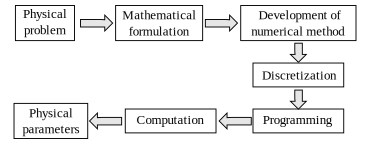
\includegraphics[scale=1]{basic.pdf}
	\end{figure}
	}	
	\subsection{Estado del arte}
	\frame{
	\frametitle{Sobre las aplicaciones de la simulación en EM}
	\begin{figure}
	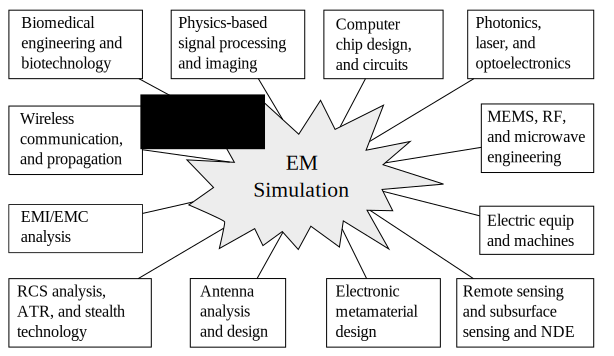
\includegraphics[scale=0.5]{EM_simulation_applications.pdf}
	\end{figure}
	}
	\frame{
	\frametitle{Estado del arte}
	Antenas sobre substratos hechos a partir de cristales fotónicos tomado de Brown y Yablanovich \cite{E.R.Brown1993a}:
	\note{Los cristales fotónicos como substrato permiten que l radiación de la antena sea dirigida exclusivamente hacia el aire, y no quede atrapada dentro del dieléctrico.}
	
	\begin{figure}
	\includegraphics[scale=0.5]{antenna_over_pc.pdf}
	%\caption{Tomado de  \cite{E.R.Brown1993a}}
	\end{figure}
	}
	
	\frame{
	
	Aplicación de cristales fotónicos 1D y 2D para fibras ópticas de nueva generación. Tomado de "Molding the flow of Light" Joannopolous \cite{Joannopoulos2008}.
	\vskip15pt
	\begin{figure}
	\includegraphics[scale=0.5]{bragg_fibers.pdf}
	%\caption{Tomado de  \cite{E.R.Brown1993a}}
	\end{figure}
	\note{ http://www.nrl.navy.mil/techtransfer/fs.php?fs_id=97}	
	}
	
	\frame{
	La selectividad de los cristales fotónicos ha sido aprovechada por Pervez y Cheng para el desarrollo de espectrómetros ópticos de bajo costo \cite{Pervez2010}.
	\vskip15pt
	\begin{figure}
	\includegraphics[scale=0.25]{spectrometer.pdf}
	\end{figure}
	}	
	
	\frame{
	\begin{columns}
		\begin{column}{0.4\textwidth}
	Beggs y White desarrollaron acoples con guías de onda hechas a partir de cristales fotónicos que permiten hacer swicheo óptico por medio del efecto termo óptico \cite{beggsdesign}
		\end{column}
		\begin{column}{0.5\textwidth}
			\begin{figure}
			\includegraphics[scale=0.25]{swiche.jpg}
			\end{figure}
			\end{column}
	\end{columns}
	}
	\frame{
	Acoplamiento de puntos cuánticos con cavidades ópticas para procesamiento cuántico de información. La transmitividad de la cavidad es controlada por el estado del punto cuántico. El estado del punto se cambia a su vez usando lasers.   \cite{AndreiFaraon2008}
	\vskip15pt
	\note{Fig. 2. Schematic showing the operation of the device. A heating laser is used to control the
device temperature thus changing the resonance frequency of the cavity and the quantum
dots coupled to it [12]. A probe laser is injected into the cavity from the top. The cavity field
couples to the waveguide mode and then it is scattered from the grating outcoupler into the
collection lens. A pinhole is used to collect only the output scattered by the grating. Using
this device, the transmission function of the cavity can be analyzed for different frequencies
of the resonator, quantum dot and probe laser.
}
	\begin{figure}
	\includegraphics[scale=0.15]{quantum_device.pdf}
	\end{figure}	
	}
\section{Marco Teórico}

	\subsection{La física detrás de un cristal fotónico}
	\frame{
	\frametitle{Las ecuaciones que rigen el problema}
	\centerline{Ecuaciones de Maxwell}
	\vskip20pt
	\begin{columns}[t]
		\begin{column}{0.5 \textwidth}
		\begin{block}{En forma Integral }
		\small
		\begin{align*}
		&\oint_C \mathbf{E}\cdot d\mathbf{l} = -\frac{d}{dt}\int_S \mathbf{B}\cdot d\mathbf{S} \\
&\oint_C \mathbf{H}\cdot d\mathbf{l} = \frac{d}{dt}\int_S \mathbf{D}\cdot d\mathbf{S} + \int_S \mathbf{J}\cdot d\mathbf{S} \\
&\int_S \mathbf{D}\cdot d\mathbf{S} = \int_V \rho dV  \\
&\int_S \mathbf{B}\cdot d\mathbf{S} = 0 
		\end{align*}
		
		\end{block}
		\end{column}
		\begin{column}{0.45 \textwidth}
		
		\begin{block}{forma diferencial}
		\small
		\begin{align*}
&\nabla\times \mathbf{E} = - \frac{\partial \mathbf{B}}{\partial t}  \\
&\nabla\times \mathbf{H} =  \frac{\partial \mathbf{D}}{\partial t} + \mathbf{J} \\
&\nabla\cdot \mathbf{D} = \rho  \\
&\nabla\cdot \mathbf{B} = 0  
		\end{align*}		
		\end{block}
		\end{column}
	\end{columns}
	}
	
	\subsection{Los métodos para simular el fenómeno}

\section{Implementación}
	\subsection{Requerimientos}
	\subsection{Pasos de desarrollo}
	\subsection{Herramientas}
	\subsection{Ejemplos, y referencias}
\section{Resultados}

\section{Conclusiones y trabajo futuro}	
	\subsection{Trabajo futuro}
	\begin{frame}
		\frametitle{Trabajo futuro}
		¿Qué vale la pena explorar en trabajos futuros?		
		\begin{itemize}
		\pause
		\item Elementos triangulares vectoriales y de segundo orden.
		\pause		
		\item  Elementos cuadrilateros lineales y escalares.
		\pause
		\item Añadir soporte para condiciones de frontera infinitas de alguno de estos tipos:
		\begin{itemize}
			\pause
			\item  Perfectly Matched Layers PML\cite{Jin2010}. 
			\pause
			\item Uso de condiciones de frontera de Robin cuando la impedancia intrínseca es conocida.
			\pause
			\item Mapeo  de la región no acotada a una geometría conocida (e.g con mapeo conformal). \pause
		\item Formulación híbrida de  FEM y Boundary Elements(BEM) como la desarrollada por Nicol\'as Guar\'in en \cite{Guarin2012}.
		\pause
		\item Elementos Infinitos, caso especial de los elementos finitos con un comportamiento de decaída (\cite{Zienkiewicz2005}).
		\end{itemize} 
	\end{itemize}
	\end{frame}
	\begin{frame}
	¿Qué vale la pena explorar en trabajos futuros?
		\begin{itemize}
		\pause
		\item Evaluar convergencia de las rutinas de solución para los problemas descritos en los resultados usando mallas más finas.
		\pause
		\item Realizar más simulaciones en el dominio del tiempo en las cuales se resuelva para defectos en cristales finitos.
		\pause
		\item Comparar los resultados de factor Q y eficiencia, con publicaciones en la literatura.
		\pause
		\item Integrar la herramienta CAD, y el solucionador en una rutina que pueda resolver problemas de optimización topológica para maximizar propiedades como confinamiento o transmisión induciendo variaciones en la posición y forma de los defectos en la red.
		\pause
		\item Implementar un esquema de paralelización.
		\pause
		\item Integración de procesos de pre y post procesamiento externos por medio de scripting que usa librerías de Python compatibles con gmsh o Paraview Python libraries.
		\end{itemize}
	\end{frame}

\section{Bibliograf\'ia}
  \begin{frame}[allowframebreaks]
  \frametitle{Bibliograf\'ia}
  \bibliographystyle{unsrt}
  \bibliography{thesis_references}
  \end{frame}

\end{document}
